\documentclass[../../main.tex]{subfiles}
\graphicspath{{\subfix{../../media/}}}


\begin{document}
	
	\begin{definition}\label{def: scalar line integration}
		Line integration of a scalar field $f: \mathbb{R}^n \rightarrow \mathbb{R}$ along a smooth curve $C$
		\begin{equation}
			\int_C f(\mathbf{x}) \; ds
		\end{equation}
	\end{definition}
				
	\par The definition above is derived from the concept of Riemann summation. To illustrate this, we will we take the following toy example.
	
	\begin{example}
		Given a scalar valued function $f(x, y) = 0.6\cos \left ( \sqrt{x^2+y^2} \right ) + 3$ and a parametric curve $C$ defined by following equations 
		\begin{align*}
			x &= 6t \cos(5t)		&&y = 6t^3 - 6\\
		\end{align*}
		Derive the definition of line integration exploiting the concept of Riemann summation. Graph some Riemann approximation of the line integration of $f(x, y)$ along curve $C$ for arbitrary $n$
	\end{example}
	\begin{solution}
		Riemann summation performed on $f(x, y)$ along curve $C$ can be achieve by the following steps:
		\begin{enumerate}
			\item Divide the curve $C$ to $n$ small subarcs\footnote{small arcs} $\Delta s_1, \dots \Delta s_n$.
			\item For every subarc $i$, evaluate $f(x,y)$ at some point\footnote{choice of $(x_i^*, y_i^*)$ will decide which Riemann sum we have. Either Right, Left, Midpoint Riemann sum} $(x_i^*, y_i^*) \in \Delta s_i$.
			\item Compute $f(x_i^*, y_i^*) \Delta s_i$ for every subarc "i.e the area of a rectangle with length $f(x_i^*, y_i^*)$ and width $\Delta s_i$ for subarc $i$".
			\item Sum $f(x_i^*, y_i^*) \Delta s_i$ over $n$ "i.e. the rectangles" to approximate the area under $f(x,y)$ along path $C$.
				\begin{equation*}
					\text{Area under the curve} \approx \sum_{i=1}^n f(x_i^*, y_i^*) \Delta s_i 
				\end{equation*}
			\item Riemann summation imply that $n$ goes to infinity "i.e. the rectangles become infinitely small". Hence the Riemann summation gives us the line integration\footnote{recall that $\int \equiv lim_{n \rightarrow \infty} \sum_{i=1}^n$} of $f(x,y)$ along curve $C$
				\begin{equation*}
					\int_C f(x, y) ds = \lim_{n \rightarrow \infty} \sum_{i=1}^n f(x_i^*, y_i^*) \Delta s_i 
				\end{equation*}
		\end{enumerate}
		
		\par For arbitrary chosen $n$, that is not too large; the Riemann sum would look rectangles that cover the area between curve $C$ and function $f(x,y)$.
			\begin{figure*}[h]
				\begin{subfigure}[c]{0.43\textwidth}
					\centering
					\begin{tikzpicture}[
							declare function={
								xs(\t) = 6*\t*cos(deg(5*\t));
								ys(\t) = 6*\t^3 - 6;
								}
							]
						\begin{axis}[
						    view = {0}{90},
					        colormap/viridis,
						  	domain=-7:7,
			  			    xmin=-7, xmax=7,
						    ymin=-7, ymax=7,
				  	        width=\linewidth
							]
						    \addplot3[contour filled={number = 50}, thick, opacity=0.8]{-0.6*cos(deg(sqrt(\x^2+\y^2))) + 3};
							
							\addplot[red, thick, samples=20, parametricmarker, samples y=0, domain=0.5:1.1, variable=\t] ({xs(\t)}, {ys(\t)});
							
							\addplot[black, thick, samples=3, samples y=0, domain=0.81:0.917, variable=\t] ({xs(\t)}, {ys(\t)});
							\node at (axis cs:-0.8,0.8) [black, anchor=north east] {$\Delta s_i$};
							
						\end{axis}
					\end{tikzpicture}
				\end{subfigure}
				\hfil
				\begin{subfigure}[c]{0.5\textwidth}
					\centering
					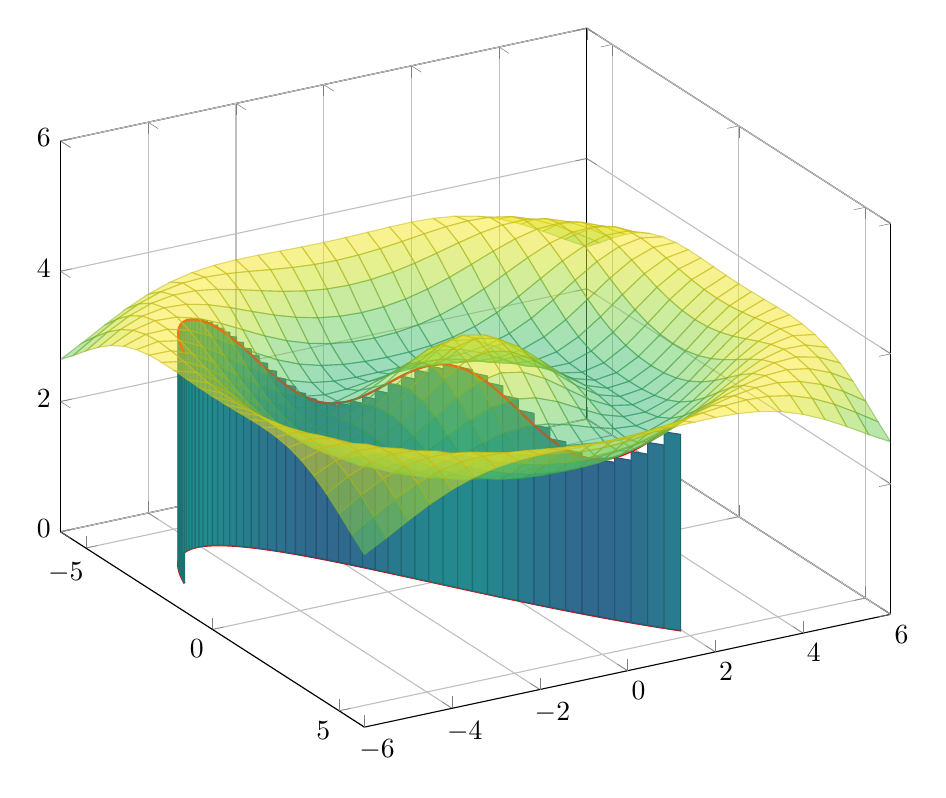
\begin{tikzpicture}[
						declare function={
							f(\x,\y) = 0.6*cos(deg(sqrt(\x^2+\y^2))) + 3;
							xs(\t) = 6*\t*cos(deg(5*\t));
							ys(\t) = 6*\t^3 - 6;
							}
						]
					    \begin{axis}[
					        view={60}{30},
					        grid=both,
					        colormap/viridis,
					        domain=-6:6,
						    xmin=-6, xmax=6,
					        ymin=-6, ymax=6,
						    zmin=0, zmax=6,
						    width=\linewidth,
						    ]
						    
						    % parametars
						    \newcommand{\h}{0.01}
		
							% parametric curve in (x,y,0) plane
							\addplot3 [red, thick, samples=100, samples y=0, domain=0.5:1.1, variable=\t] ({xs(\t)}, {ys(\t)}, 0);						
							\pgfplotsinvokeforeach{0.5,0.5+\h,...,1.1-\h}{
			    					\addplot3 [red, patch, patch type = rectangle] coordinates {
										({xs(#1)}, {ys(#1)}, 0) 
										({xs(#1+\h)}, {ys(#1+\h)}, 0) 
										({xs(#1+\h)}, {ys(#1+\h)}, {f(xs(#1),ys(#1))}) 
										({xs(#1)}, {ys(#1)}, {f(xs(#1),ys(#1))})
										};
							}
							\addplot3 [red, thick, samples=100, samples y=0, domain=0.5:1.1, variable=\t, point meta=0] ({xs(\t)}, {ys(\t)}, {f(xs(\t), ys(\t))});
													
							% function
							\addplot3 [surf, opacity=0.5] {f(\x,\y)};	
			
					    \end{axis}
					\end{tikzpicture}
				\end{subfigure}
				\caption{Left: Illustrating $\Delta s_i$. Right: Riemann summation for small $n$}
			\end{figure*}
		The plot above is the approximated line integration of $f(x,y)$ along curve $C$ using Riemann sum.
	\end{solution}
	
	\par In context of parametric curves, it is more convenient\footnote{computationally} to reformulate line integration formula  "presented in definition (\ref{def: scalar line integration})" in terms integration operator for the parametric variable "usually referred as $t$" rather than the arc length "usually referred as $s$" hence $ds \rightarrow dt$.
	
	\begin{definition}
		Line integration of a scalar field $f: \mathbb{R}^2 \rightarrow \mathbb{R}$ along a smooth parametric curve curve $C$ that defined by variable $t$
		\begin{equation*}
			\int_C f(x,y) ds = \int_a^b f(x(t), y(t)) \sqrt{\left( \frac{dx}{dt} \right)^2 + \left( \frac{dy}{dt} \right)^2} dt
		\end{equation*}
		given that
		\begin{equation*}
			\frac{ds}{dt} = \sqrt{\left( \frac{dx}{dt} \right)^2 + \left( \frac{dy}{dt} \right)^2}
		\end{equation*}
		This definition can be generalized to $\mathbb{R}^n$
	\end{definition}


	\begin{example}
		Evaluate $\int_C (2+x^2y) ds$, where $C$ is the upper half of the unit circle $x^2 + y^2 = 1$.
	\end{example}
	\begin{solution}
		The upper half of the unit circle can be expressed using the parametric curve defined by the following equations
		\begin{align*}
			x &= \cos t		&&y = \sin t\\
		\end{align*}
		Hence the line integral reads
		\begin{align*}
			\int_C (2+x^2y) ds 	&= \int_0^\pi (2 + \cos^2t \sin t) \sqrt{\left( \frac{dx}{dt} \right)^2 + \left( \frac{dy}{dt} \right)^2} dt \\
								&= \int_0^\pi (2 + \cos^2t \sin t) \sqrt{\sin^2 t + \cos^2 t} dt \\
								&= \int_0^\pi (2 + \cos^2t \sin t) dt\\
								&= \left\lbrack 2t - \frac{cos^3 t}{3}  \right\rbrack_0^\pi = 2\pi + \frac{2}{3}
		\end{align*}
	\end{solution}
		
\end{document}